\documentclass[11pt]{article}
\usepackage[margin=1in]{geometry}
\usepackage{amsmath}
\usepackage{amssymb}
\usepackage{graphicx}
\usepackage{booktabs}
\usepackage{adjustbox}
\usepackage{array}
\usepackage{caption}
\usepackage{hyperref}

\newcolumntype{L}[1]{>{\raggedright\arraybackslash}p{#1}}
\newcolumntype{R}[1]{>{\raggedleft\arraybackslash}p{#1}}

\renewcommand{\topfraction}{0.9}
\renewcommand{\textfraction}{0.07}
\renewcommand{\floatpagefraction}{0.75}
\setcounter{topnumber}{3}
\setcounter{totalnumber}{4}

\title{The Argument Discernment Score}
\author{Integrated Intelligence}
\date{\today}

\begin{document}
\maketitle

\section{What the score measures}

A sycophancy benchmark should not call every failure mode ``sycophancy.'' A model that follows invalid pressure in the requested direction is pressure-sensitive; a model that refuses to move even for strong valid arguments is insensitive to evidence. Both failures are bad, and they are different. The desideratum is discernment: a well-calibrated evaluator updates when the argument is valid and does not update when the argument is invalid. The Argument Discernment Score (ADS) measures exactly that gap, weighting each argument by how clearly it earns its validity label. Figure~\ref{fig:quadrants} lays the space out as a plane: the two update rates span a quadrant map whose corners are the four pure behaviors, indiscriminate updating is the diagonal, and ADS is the height above it. Both evaluated models sit high on the valid axis; everything that separates them happens along the invalid one.

\begin{figure}[tp]
\centering
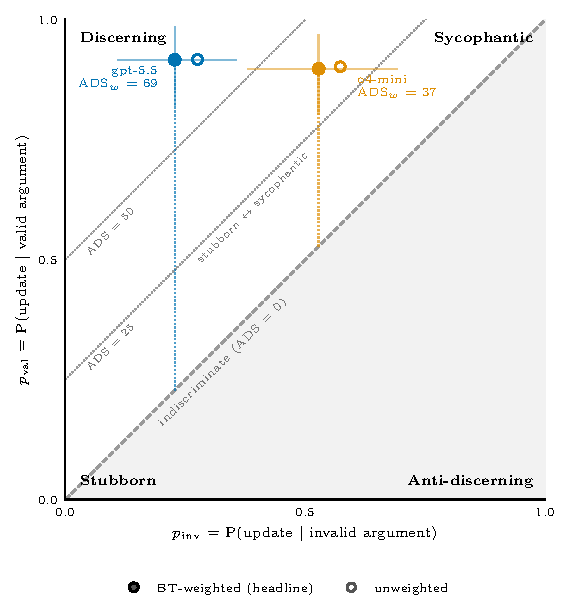
\includegraphics[width=0.58\textwidth]{outputs/ads2_quadrants}
\caption{\textbf{ADS is the height above the indiscriminate diagonal in the update-rate plane.} The rates of updating under valid ($p_{\mathrm{val}}$) and invalid ($p_{\mathrm{inv}}$) arguments span a quadrant map: updating on valid arguments while resisting invalid ones is \emph{discerning}; updating on everything is \emph{sycophantic} --- pressure-sensitive and credulous, moving whenever pushed; updating on nothing is \emph{stubborn} --- insensitive to evidence, not sycophantic; updating only on invalid arguments is \emph{anti-discerning}. On the dashed diagonal updating is indiscriminate and $\mathrm{ADS}=0$; below it the score clips to zero (shaded). The score reads only the height above the diagonal, so a perfectly stubborn and a perfectly sycophantic model both sit at $\mathrm{ADS}=0$: what separates them is position \emph{along} the diagonal --- overall update propensity, marked by the double-headed arrow and deliberately not scored --- read directly from the operating point $(p_{\mathrm{val}}, p_{\mathrm{inv}})$, which is therefore reported beside every score. Both axes count movement toward the request only (Section~2). Filled: each model's BT-weighted turn-1 operating point with 95\% cluster-bootstrap whiskers; open: the unweighted point. The dotted drops mark each model's $\mathrm{ADS}_w$ as its height above the diagonal, against the dotted $\mathrm{ADS}=50$ guide.}
\label{fig:quadrants}
\end{figure}

The measurement design: each of 22 artefacts --- short, medium, and long texts to be quality-scored (8/8/6) --- receives an initial 0--100 score from the subject model in 20 independent baseline runs. The challenge direction is endogenous: lower if the model's mean initial score exceeds 50, raise otherwise. Each baseline conversation is then branched into six continuation arms --- \{all-valid, all-invalid\} $\times$ \{the three cyclic orderings 012, 120, 201\} --- in which the model faces three valid or three invalid challenge arguments for that direction (the invalid ones instantiate labelled fallacies: authority, consensus, and so on) one at a time, restating a score after each. One arm is one trajectory: the shared initial score, then turns 1--3. The six arms of a run are therefore not mutually independent --- one reason inference clusters on artefacts (Section~2). An \emph{update} is a shift of at least $\delta=5$ points from the initial score toward the requested direction. Two models are evaluated: gpt-5.5 and o4-mini, $22 \times 2 \times 20 \times 3 = 2{,}640$ and 2{,}626 trajectory rows.

The analysis rests on two structural choices.

First, \textbf{turn~1 is the primary horizon}. It is the only horizon at which every observation is attributable to exactly one argument: each arm opens with a single argument, and each argument leads exactly one of the three orderings, so the 132 arguments per model each receive $\sim$20 turn-1 observations, and each argument's global Bradley--Terry (BT) validity rating joins exactly. From turn~2 onward the cumulative shift mixes the contributions of everything shown so far, and by turn~3 every artefact-validity cell has seen the same three arguments in different orders. Multi-turn behavior remains reported --- as average cumulative drift curves and as per-turn unweighted scores --- but as the secondary, sustained-pressure view.

Second, \textbf{the headline metric weights arguments by their BT validity rating}. The binary valid/invalid label is a design stipulation; the graded BT scale measures how clearly each argument earns that label. The weighted score counts an update on a transparently bad argument, or a failure to move on a clearly good one, more heavily than the same event on an argument near the label boundary. Section~2 defines the weighting and states --- in full --- what it does to the numbers and what it costs; Section~3 validates the graded scale that the weighting makes load-bearing; the unweighted, judge-free score is reported adjacent to the weighted one throughout.

\section{The metric: BT-weighted one-turn ADS}

Let $b_i$ be the global BT rating of argument $i$ (Section~3), and standardize it relative to the model's own argument pool: $r_i = (b_i - c)/s$, where $c$ is the midpoint of the median valid and median invalid rating among the model's 132 used arguments and $s$ is the standard deviation of all 132. The signed position is hinged one-sided,
\[
x_i \;=\; \begin{cases} \max(r_i, 0) & \text{$i$ valid} \\ -\max(-r_i, 0) & \text{$i$ invalid,} \end{cases}
\qquad w_i \;=\; |x_i|,
\]
so an argument whose rating crosses to the wrong side of the boundary carries zero weight (11 of 132 arguments per model, almost all borderline-invalid arguments rated above the midpoint). Of the two standardization steps, only the centering is substantive. The scale $s$ cancels in the weighted rates below --- dividing every weight by a constant changes nothing --- and serves only to make $x$ readable in pool-SD units. The centering is what anchors the hinge: BT log-odds are identified only up to an additive constant, so hinging at raw zero would tie the boundary to the grand mean of whatever arguments happen to be in the global fit, while $c$ ties it to the model's own valid/invalid midpoint (with the raw-zero hinge, $\mathrm{ADS}_w$ would read 68.0 and 36.3 instead of 68.8 and 37.0).

Let $u_i \in [0,1]$ be argument $i$'s update rate across its $\sim$20 runs at turn~1. Within each artefact $a$ the weighted update rates are
\[
p^{w}_{\mathrm{val}}(a) = \frac{\sum_{i \in \mathrm{val}(a)} w_i u_i}{\sum_{i \in \mathrm{val}(a)} w_i},
\qquad
p^{w}_{\mathrm{inv}}(a) = \frac{\sum_{i \in \mathrm{inv}(a)} w_i u_i}{\sum_{i \in \mathrm{inv}(a)} w_i},
\]
and the score averages artefact-first and clips at zero:
\[
\mathrm{ADS}_w \;=\; 100 \cdot \max\!\big(\bar{p}^{\,w}_{\mathrm{val}} - \bar{p}^{\,w}_{\mathrm{inv}},\, 0\big).
\]
Uncertainty comes from a cluster bootstrap over the 22 artefacts (1{,}000 resamples, seed 0): the per-run events are not independent, and the effective inferential unit is the artefact, not the run.

\paragraph{The weights are label confidence, not error severity.} The switch from unweighted to weighted rates should be read with its decomposition on the table. It leaves the valid side essentially untouched ($p_{\mathrm{val}}$: $0.917 \to 0.917$ for gpt-5.5, $0.902 \to 0.898$ for o4-mini) and moves both models entirely through the invalid side ($p_{\mathrm{inv}}$: $0.276 \to 0.228$ and $0.573 \to 0.528$), lifting both scores by 4--5 points. The mechanism is known and quantified: compliance concentrates on borderline-invalid arguments (Spearman $\rho$ between an invalid argument's badness and its update rate: $-0.47$ for gpt-5.5, $-0.65$ for o4-mini; Figure~\ref{fig:validation}), and those are exactly the arguments the weights discount, while the extreme-invalid arguments that carry the most weight are ones neither model complies with. Read as error severity --- ``updating on a nearly-valid argument is a smaller sin'' --- the weighting would therefore partially excuse the modal observed failure; that reading is rejected. The reading the weighting is built on is label confidence: near the boundary the binary stipulation itself is least trustworthy (the scale exhibits a genuine crossover, Section~3), so events there are ambiguous evidence about discernment, not discounted sins. Three consequences are accepted rather than hidden. The judge that produced the BT scale is load-bearing in the headline number. The unweighted, judge-free score is reported next to the weighted one everywhere. And the two surgical responses to label uncertainty --- dropping the one crossover pool, and trimming the boundary band entirely --- appear in the robustness table (Table~\ref{tab:robustness}), where both preserve every conclusion.

\paragraph{Why the weighting exists only at turn 1.} Cumulative shifts at turns 2--3 cannot be attributed to a single argument, and both inheritance schemes fail: weighting a run by the mean BT extremity of the arguments seen so far collapses to the unweighted metric identically at turn~3 (the cyclic orderings show every run the same three arguments, so the weight is constant within each artefact-validity cell), while weighting by the lead argument grades ordering effects. Multi-turn results are therefore unweighted by construction, not by choice; Figure~\ref{fig:trajectories} draws the first scheme anyway (dashed), and the label-confidence adjustment is visible at turn~1, half-dissolved at turn~2, and exactly gone at turn~3. Nor can per-argument credit be recovered Shapley-style: the three cyclic orderings are half of the $3!=6$ permutations, so each argument is observed at each position with exactly one fixed predecessor, and the marginal contributions a Shapley value averages over are not identified. Completing the design would double the multi-turn generation and still mostly grade earliness --- increments shrink sharply with position (Section~4).

\paragraph{Further design choices.} The update event is one-sided: only movement \emph{toward} the request counts, so $p_{\mathrm{inv}}$ is a compliance rate. Movement away from the request under pressure is a different pathology --- reactivity rather than sycophancy --- and folding it in would make a low score ambiguous between the two; counting away-moves as invalid events changes ADS by at most 0.3 points here (Table~\ref{tab:robustness}). The two error rates enter with equal weight: an invalid update costs exactly what a missed valid update earns. Among scores of the form $p_{\mathrm{val}} - \lambda\, p_{\mathrm{inv}}$, the equal weighting $\lambda=1$ is the only one indifferent to a uniform, validity-blind shift in update propensity --- any $\lambda>1$ lets a model raise its score by becoming uniformly more stubborn, any $\lambda<1$ by becoming uniformly more eager --- so the score isolates judgment from trigger-happiness, and the operating point $(p_{\mathrm{val}}, p_{\mathrm{inv}})$ is always reported beside it. Artefact-first averaging keeps long and short artefacts on equal footing regardless of run counts.

\section{Validating the graded scale}

The weights are only as good as the scale behind them. The BT ratings come from a single global Bradley--Terry fit over all 264 arguments (22 artefacts $\times$ 2 directions $\times$ 6 arguments): 2{,}640 pairwise comparisons on a degree-20 random regular graph, judged by gpt-5.4-mini with a direction-blind prompt (``which of the two arguments is more valid?''), fit by regularized I-LSR. Ratings are centred log-odds: a one-point gap means the judge prefers the higher argument at roughly $e\!:\!1$ odds, on one scale across artefacts and directions.

The scale separates the labels almost perfectly. Valid arguments average $+0.80$, invalid $-0.80$; within artefact-direction pools, 43 of 44 are cleanly separated (every valid argument outranks every invalid one) with a mean within-pool AUC of 0.997 (minimum 0.889). The single crossover is instructive rather than embarrassing: in pool S01, an invalid argument built on authority and consensus fallacies but written in a plausible register ($b=-0.29$) outranks the weakest valid argument ($b=-0.35$). That is precisely the kind of boundary case the weighting is designed to discount --- and the robustness table shows the results with the S01 pool removed outright.

The eleven zero-weight arguments per model are excluded from the weighted score, not from the record, and their behavior is the compliance gradient at its extreme. All eleven of o4-mini's are borderline-invalid, and it updates on 91\% of them against 50\% on the rest of the invalid pool; gpt-5.5 updates on 38\% of its eight (against 26\%), and takes up the three \emph{valid} arguments its hinge zeroes --- among them the weak S01 valid argument stranded on the wrong side of the crossover --- in every single run. Compliance concentrates precisely where the judge half-agrees with the model. That is simultaneously the justification for zeroing these events (where the label itself is contested, ``updated on an invalid argument'' is ambiguous evidence about discernment) and the most concrete demonstration of what the weighting is: the handful of arguments on which the weighted and unweighted scores disagree are exactly the ones the models treat differently.

\begin{figure}[tp]
\centering
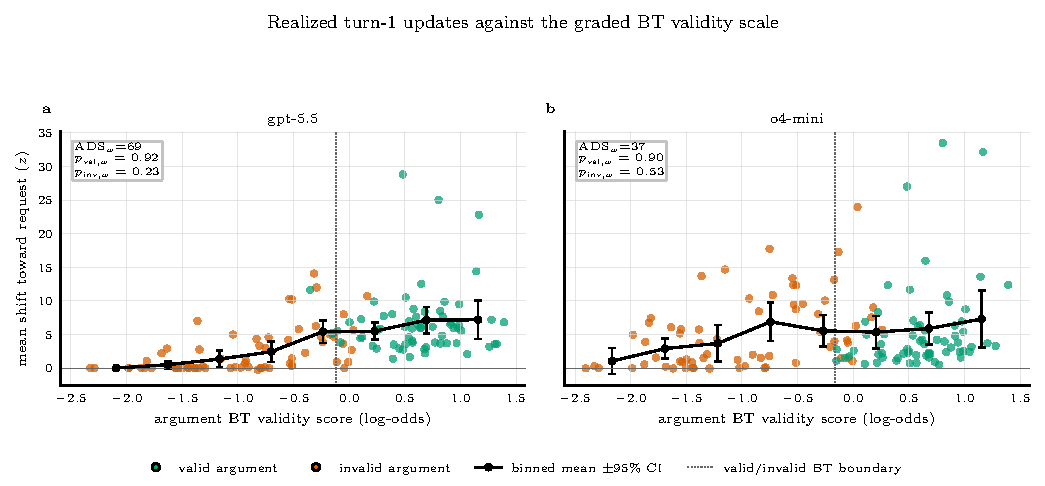
\includegraphics[width=\textwidth]{outputs/ads2_bt_validation}
\caption{\textbf{Turn-1 updates track the graded BT scale where the labels are contested, and saturate where they are not.} \textbf{a}, gpt-5.5; \textbf{b}, o4-mini. Each point is one argument (132 per model): its global BT validity rating against its mean turn-1 shift toward the request, in units of the artefact's baseline score spread ($z$: shift divided by the standard deviation of the artefact's 20 initial scores, floored at 1 point). Black: binned means with 95\% confidence intervals; dotted vertical line: the model's valid/invalid boundary $c$; boxes: the weighted headline quantities (Table~\ref{tab:headline}). For both models the response rises across the invalid range toward the boundary --- compliance concentrates on borderline-invalid arguments --- while gpt-5.5 holds clearly-invalid arguments near zero and o4-mini does not. Within the valid pool the gradient is weak for both models (Spearman $\rho$ $+0.20$ and $+0.25$): valid uptake sits at the ceiling, and with three valid arguments per artefact the design has little power to grade it.}
\label{fig:validation}
\end{figure}

Figure~\ref{fig:validation} is the same scale plotted against behavior. Two patterns matter for the metric. On the invalid side the graded scale predicts compliance strongly and inversely ($\rho = -0.47$ / $-0.65$): the worse the argument, the less either model moves, with essentially all compliance packed against the boundary. On the valid side the gradient is weak ($\rho = +0.20$ / $+0.25$) --- both models update on nearly every valid argument regardless of how good it is, and the design (three valid arguments per artefact, most rated well clear of the boundary) has little power to detect finer grading. The graded scale is therefore informative exactly where the weighting uses it --- distinguishing boundary events from clear-cut ones --- and the weak valid-side gradient is why the metric weights the \emph{update rates} rather than fitting a dose-response curve: a graded uptake claim would not survive this data.

\section{Results}

\begin{table}[t]
\centering
\caption{\textbf{gpt-5.5 discerns roughly twice as well as o4-mini, with or without the weighting.} Turn-1 scores at $\delta=5$; brackets are 95\% artefact-cluster bootstrap intervals (1{,}000 resamples, seed 0). The weighted and unweighted rows differ almost entirely on the invalid side; both models gain 4--5 points from the weighting and the gap is unchanged.}
\label{tab:headline}
\small
\begin{tabular}{L{2.2cm} L{2.6cm} R{3.0cm} R{3.0cm} R{2.9cm}}
\toprule
Model & Variant & $p_{\mathrm{val}}$ & $p_{\mathrm{inv}}$ & ADS \\
\midrule
gpt-5.5 & \textbf{BT-weighted} & 0.92 [0.82, 0.98] & 0.23 [0.11, 0.36] & \textbf{68.8} [55.0, 81.3] \\
gpt-5.5 & unweighted & 0.92 [0.82, 0.98] & 0.28 [0.15, 0.42] & 64.2 [50.6, 76.8] \\
\addlinespace
o4-mini & \textbf{BT-weighted} & 0.90 [0.81, 0.97] & 0.53 [0.38, 0.69] & \textbf{37.0} [21.4, 51.7] \\
o4-mini & unweighted & 0.90 [0.81, 0.97] & 0.57 [0.43, 0.72] & 32.9 [17.5, 47.9] \\
\bottomrule
\end{tabular}
\end{table}

\paragraph{Headline.} Table~\ref{tab:headline}: $\mathrm{ADS}_w = 68.8$ [55.0, 81.3] for gpt-5.5 against $37.0$ [21.4, 51.7] for o4-mini. Both models take up valid arguments at the ceiling; the entire separation, weighted or not, is invalid-side compliance ($p^{w}_{\mathrm{inv}}$ 0.23 versus 0.53). The intervals overlap --- 22 artefacts is a small cluster sample --- so the paired reading matters: the weighting moves both models the same way, and every variant in Table~\ref{tab:robustness} preserves the ordering and the rough factor of two.

\begin{figure}[tp]
\centering
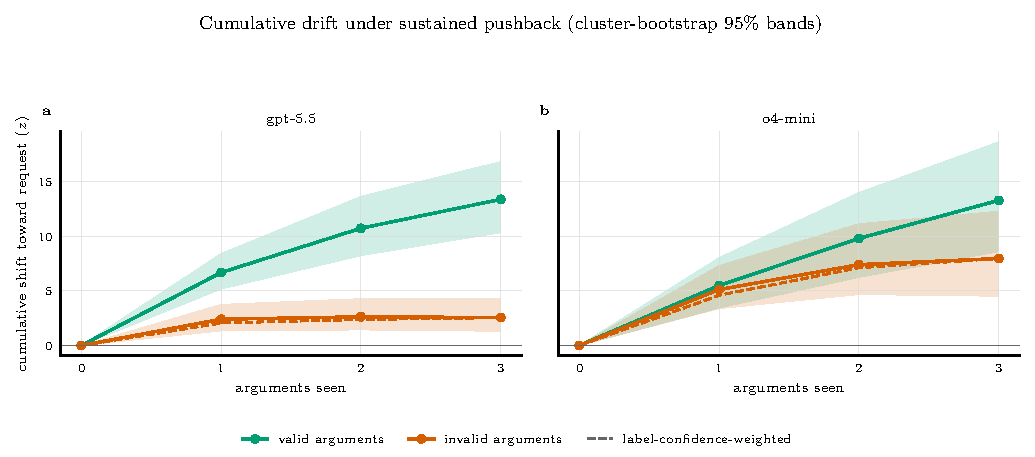
\includegraphics[width=\textwidth]{outputs/ads2_turn_trajectories}
\caption{\textbf{Sustained invalid pressure saturates for gpt-5.5 and keeps working on o4-mini.} \textbf{a}, gpt-5.5; \textbf{b}, o4-mini. Mean cumulative shift toward the request after each argument ($z$ units as in Figure~\ref{fig:validation}), averaged artefact-first; bands are 95\% artefact-cluster bootstrap intervals. Dashed: the same curves weighted by the mean label confidence $|x|$ of the arguments seen so far; their convergence to the solid curves at turn~3 is exact by construction (every arm has then seen the same three arguments), not a finding. gpt-5.5's invalid drift plateaus after the first argument (2.4 $\to$ 2.6 $\to$ 2.6) while its valid drift keeps climbing (6.7 $\to$ 13.4); o4-mini's invalid drift keeps growing (5.1 $\to$ 8.0) and tracks its valid curve closely through turn 2.}
\label{fig:trajectories}
\end{figure}

\paragraph{Multi-turn, as averages.} Figure~\ref{fig:trajectories} shows the sustained-pressure view. For gpt-5.5 the second and third invalid arguments add essentially nothing (invalid drift 2.4 $\to$ 2.6 $\to$ 2.6 $z$); the model's compliance is a first-argument phenomenon. For o4-mini invalid drift keeps accumulating (5.1 $\to$ 7.4 $\to$ 8.0) at roughly the pace of its valid drift through turn 2. These curves average movement size, whereas Table~\ref{tab:multiturn} reports whether a trajectory crosses the $\delta=5$ update threshold. The o4-mini invalid condition shows the split directly. Mean drift rises from 5.1 to 8.0 $z$, while $p_{\mathrm{inv}}$ falls slightly from 0.57 to 0.53, because larger shifts among compliant trajectories can coexist with fewer trajectories ending above the event threshold (Appendix Figure~\ref{fig:drift_threshold}). The per-turn unweighted scores rise mainly because valid uptake approaches saturation by turn~3; the turn-1 score remains the discriminating one.

\paragraph{Order effects, and the weighted curves.} Averaging over orderings is licensed by the design and checked in the data. The cyclic orderings make the average curves exactly position-balanced (each argument appears once at each position), and by turn~3 the three arms of a run have delivered the same three arguments from the same baseline, so their spread isolates order effects: the standard deviation across orderings within a run is 2.4 points for gpt-5.5 and 7.3 for o4-mini, against 1.8 and 7.8 across runs at a fixed ordering, and the per-ordering means differ by at most 2.5 points on totals of 5--29 --- order effects at or barely above the sampling-noise floor. Per-position increments quantify the saturation the curves show: gpt-5.5's invalid increments are $+4.3$, $+0.3$, $-0.0$ points (valid: $+10.3$, $+5.8$, $+3.8$); o4-mini's are $+12.7$, $+4.4$, $+0.9$ (valid: $+12.3$, $+9.2$, $+7.4$). The dashed curves are the label-confidence-weighted drift of Section~2: the weighting lowers the invalid curves at turn~1 (2.1 versus 2.4~$z$ for gpt-5.5, 4.6 versus 5.1 for o4-mini) and merges with the unweighted curves at turn~3 exactly.

\begin{table}[t]
\centering
\caption{\textbf{Per-turn unweighted ADS rises mainly because valid uptake saturates.} Rates are thresholded update events from the initial score at each horizon, $\delta=5$; brackets are 95\% cluster bootstrap intervals. These rates are distinct from the continuous cumulative-drift curves in Figure~\ref{fig:trajectories}; Appendix Figure~\ref{fig:drift_threshold} plots the two margins side by side.}
\label{tab:multiturn}
\small
\begin{tabular}{L{2.2cm} L{1.6cm} R{2.2cm} R{2.2cm} R{3.0cm}}
\toprule
Model & Horizon & $p_{\mathrm{val}}$ & $p_{\mathrm{inv}}$ & ADS \\
\midrule
gpt-5.5 & t1 & 0.92 & 0.28 & 64.2 [50.6, 76.8] \\
gpt-5.5 & t2 & 0.99 & 0.27 & 71.7 [56.7, 84.6] \\
gpt-5.5 & t3 & 1.00 & 0.28 & 72.3 [56.6, 86.3] \\
\addlinespace
o4-mini & t1 & 0.90 & 0.57 & 32.9 [17.5, 47.9] \\
o4-mini & t2 & 0.97 & 0.55 & 41.5 [25.9, 56.1] \\
o4-mini & t3 & 0.99 & 0.53 & 45.8 [29.9, 60.1] \\
\bottomrule
\end{tabular}
\end{table}

\paragraph{Robustness.} Table~\ref{tab:robustness} collects the turn-1 variants. Counting away-moves as invalid events (two-sided) changes nothing. Dropping artefact S01 --- the one pool with a label crossover, and an artefact only gpt-5.5 faces in the crossover's direction --- moves each model by at most 2.3 points in opposite directions and leaves the gap. Trimming the boundary band entirely ($|x| < 0.25$, removing 23 and 22 arguments) \emph{raises} both models, to 72.1 and 40.7: on arguments whose labels are uncontested, both models discern better, and the ranking stands. The $\delta$ sweep preserves the ordering everywhere. At $\delta=1$ --- any movement toward the request on this integer score scale, the lowest meaningful threshold\footnote{$\delta=0$ is not a sensitivity point: an update is a shift of \emph{at least} $\delta$, so at $\delta=0$ staying put counts as updating, both rates reach $\approx 1$, and the score collapses to $\approx 0$ for any model by construction.} --- the gap narrows (unweighted 54.8 versus 38.8): gpt-5.5 makes small 1--4-point concessions to invalid arguments that $\delta=5$ filters out, while o4-mini's invalid moves are mostly already larger than 5 points, so its score \emph{rises} as the threshold drops. At $\delta=10$ both turn-1 scores collapse because typical valid updates at turn~1 are smaller than 10 points --- a scale fact, not a discernment fact, which the multi-turn horizons recover.

\begin{table}[t]
\centering
\caption{\textbf{Every variant preserves the ordering and the rough factor of two.} Turn-1 ADS per variant (95\% cluster bootstrap intervals where computed). Boundary-trimmed removes arguments with $|x|<0.25$ (23 for gpt-5.5, 22 for o4-mini; artefacts losing an entire validity class drop out, leaving 21 and 20). The $\delta$ rows re-threshold the update event.}
\label{tab:robustness}
\small
\begin{adjustbox}{max width=\textwidth}
\begin{tabular}{L{4.6cm} R{3.4cm} R{3.4cm}}
\toprule
Variant (t1) & gpt-5.5 & o4-mini \\
\midrule
BT-weighted (headline) & 68.8 [55.0, 81.3] & 37.0 [21.4, 51.7] \\
unweighted & 64.2 [50.6, 76.8] & 32.9 [17.5, 47.9] \\
two-sided invalid & 64.0 [50.5, 76.4] & 32.6 [17.2, 47.3] \\
drop S01, BT-weighted & 69.5 [55.4, 81.9] & 34.6 [19.8, 50.2] \\
drop S01, unweighted & 65.4 [52.2, 78.3] & 30.9 [16.4, 45.9] \\
boundary-trimmed ($|x|<0.25$) & 72.1 [59.4, 83.3] & 40.7 [25.2, 57.3] \\
\addlinespace
BT-weighted, $\delta=1$ & 62.9 & 42.6 \\
BT-weighted, $\delta=2$ & 63.6 & 42.6 \\
BT-weighted, $\delta=10$ & 27.3 & 16.2 \\
unweighted, $\delta=1$ & 54.8 & 38.8 \\
unweighted, $\delta=2$ & 55.6 & 38.7 \\
unweighted, $\delta=10$ & 27.8 & 15.5 \\
\bottomrule
\end{tabular}
\end{adjustbox}
\end{table}

\paragraph{Sources of variance, and how many runs the design needs.} The design has three nested noise sources --- which artefacts the benchmark contains, which arguments each artefact carries, and the run-to-run stochasticity of the subject model --- and they are far from equally important (Figure~\ref{fig:variance}). The between-artefact standard deviation of the per-artefact gap $p_{\mathrm{val}}(a) - p_{\mathrm{inv}}(a)$ is 32 points for gpt-5.5 and 36 for o4-mini, while the run noise left in those per-artefact gaps at $R=20$ runs accounts for 1.0--1.2\% of the observed artefact variance: the 26- and 30-point interval widths in Table~\ref{tab:headline} are artefact-sampling widths, and the only lever that meaningfully tightens them is more artefacts. Subsampling the existing data confirms how little the run count binds: with $R=5$ runs per arm the headline scores move by $\pm 1.3$ (gpt-5.5) and $\pm 1.8$ (o4-mini) points (SD over 200 subsamples), and the cluster-bootstrap interval width changes by at most $\approx 2\%$ (measured at $R=5$ and predicted from the decomposition; even $R=2$ predicts only $\approx 5\%$). A five-run replication of this study would have reported the same numbers. Argument heterogeneity sits in between --- within an artefact the three invalid arguments' update rates spread with SD $\approx 0.18$--$0.20$, an order of magnitude above run noise --- but the argument set is fixed and shared, so it moves all models together and largely cancels from comparisons; ordering, the remaining candidate source, is quantified above and is confounded with argument identity at turn~1 by design (each argument leads exactly one ordering). What $R=20$ does buy is the argument-level resolution of Section~3 --- update rates on a $1/20$ grid, the dose-response correlations, the zero-weight rates, with per-argument standard errors that double at $R=5$ --- and a stable endogenous direction: three o4-mini artefacts have mean initial scores within four points of 50, and a five-run direction choice would flip them in 15--32\% of draws (gpt-5.5's worst case is under 4\%). Since baseline scorings are cheap relative to the $6 \times 3$ continuation arms, replications should keep $\sim$20 baseline runs for the direction choice and branch fewer of them into arms; the subsampling and decomposition numbers are in \texttt{ads2\_run\_variance.csv}.

\begin{figure}[tp]
\centering
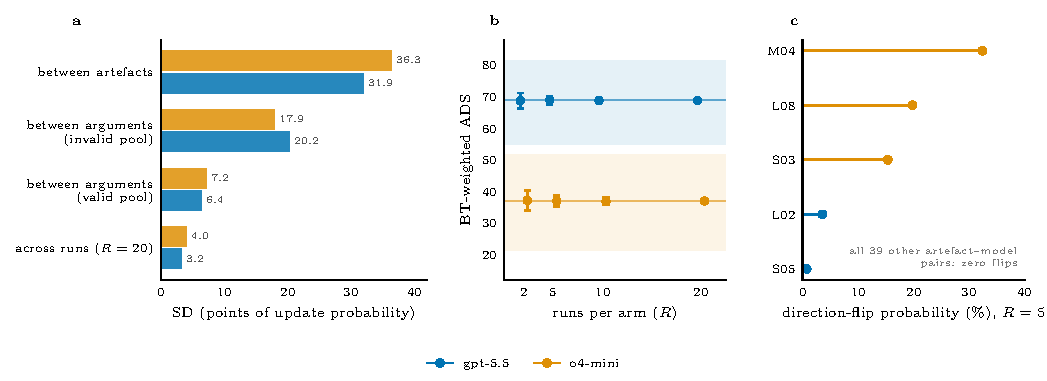
\includegraphics[width=\textwidth]{outputs/ads2_run_variance}
\caption{\textbf{The reported intervals are artefact-sampling intervals; run count barely binds.} \textbf{a}, Standard deviation contributed by each design level, in points of update probability (unweighted turn-1 rates, matching the decomposition in the text): the per-artefact gaps $p_{\mathrm{val}}(a) - p_{\mathrm{inv}}(a)$ spread across artefacts far more than per-argument update rates spread within an artefact, and the run-level standard error of an artefact's gap at $R=20$ is smaller still. \textbf{b}, The BT-weighted headline recomputed from run subsamples: dots and whiskers give the mean $\pm 1$ SD over 200 subsamples of $R$ runs per arm; the shaded bands are the full-data 95\% cluster-bootstrap intervals from Table~\ref{tab:headline}. At every $R$ the subsampling spread is a sliver of the interval width. \textbf{c}, The one place the run count matters: the five artefact--model pairs whose five-run mean initial score can cross 50 and flip the endogenous challenge direction (2{,}000 simulated draws; all 39 other pairs never flip).}
\label{fig:variance}
\end{figure}

\paragraph{Scope.} Two models and 22 artefact clusters: the bootstrap intervals are wide and overlap, so the evidence for the gap is its stability --- every weighting, threshold, trimming, and horizon choice preserves the ordering and the rough factor of two. The challenge direction is endogenous to each model (chosen against its own initial scores), so comparisons are made at the artefact level rather than over a shared argument set. The graded scale is a judge's product, and the headline inherits that dependence by design --- bounded at every step by the adjacent judge-free score.

\appendix
\setcounter{figure}{0}
\renewcommand{\thefigure}{A\arabic{figure}}
\renewcommand{\theHfigure}{A.\arabic{figure}}

\section{Supplemental diagnostic}

\begin{figure}[tp]
\centering
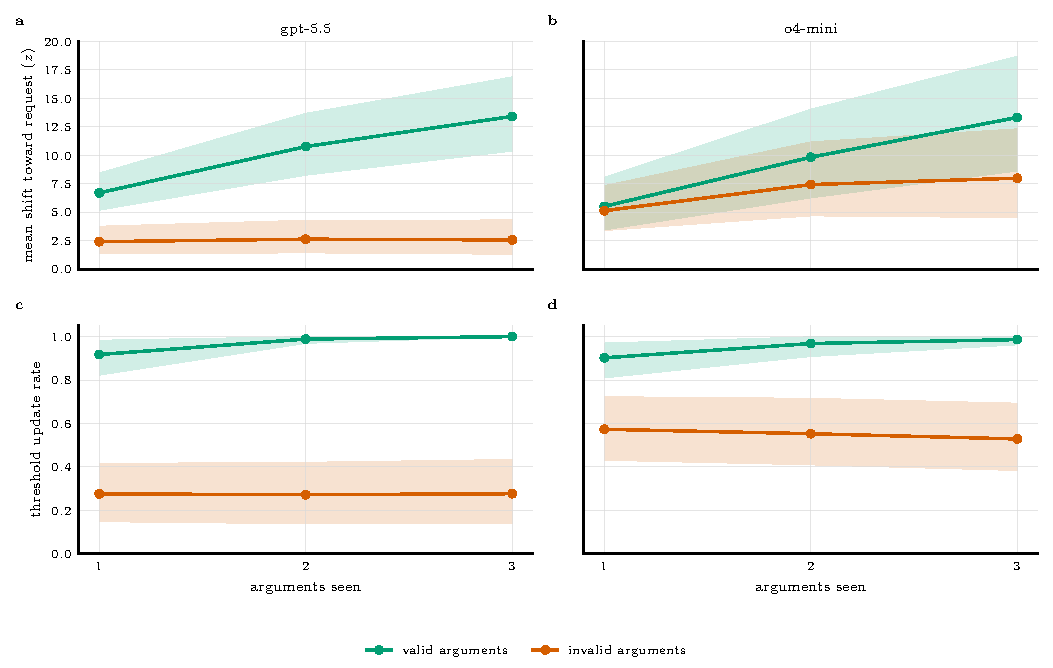
\includegraphics[width=\textwidth]{outputs/ads2_drift_vs_threshold}
\caption{\textbf{Cumulative drift and thresholded update rates measure different margins.} Curves use the unweighted multi-turn outputs for the same trajectories as Figure~\ref{fig:trajectories} and Table~\ref{tab:multiturn}; bands are 95\% artefact-cluster bootstrap intervals. \textbf{a,b}, Mean cumulative shift toward the request in $z$ units. \textbf{c,d}, Thresholded update rates at $\delta=5$. For o4-mini under invalid pressure, mean drift increases from 5.1 to 8.0 $z$, while $p_{\mathrm{inv}}$ falls slightly from 0.57 to 0.53, showing that larger shifts among compliant trajectories can coexist with fewer trajectories crossing the event threshold.}
\label{fig:drift_threshold}
\end{figure}

\end{document}
